\section{Deep Parameter Optimisation}

Our approach takes three steps. Firstly we apply Mutation Operators to generate variants of the original \emph{dlmalloc} in order to understand which pieces of the source code could be more influential to the performance. Secondly we analyze the sensitivity of each mutated piece by evaluating the variants on a given set of applications and testsuites. After locating the most interesting and influential part of the code, we expose them to users so that they could be modified from the outside as needed. Thirdly, we apply SBSE approach to find the optimal values for both the existing and exposed parameters for each of the given applications.This section first discusses how we find and expose interesting parameters.

%** maybe need add some think to justiy the choice of self-implementation. 

\begin{figure}[htbp]
\centering
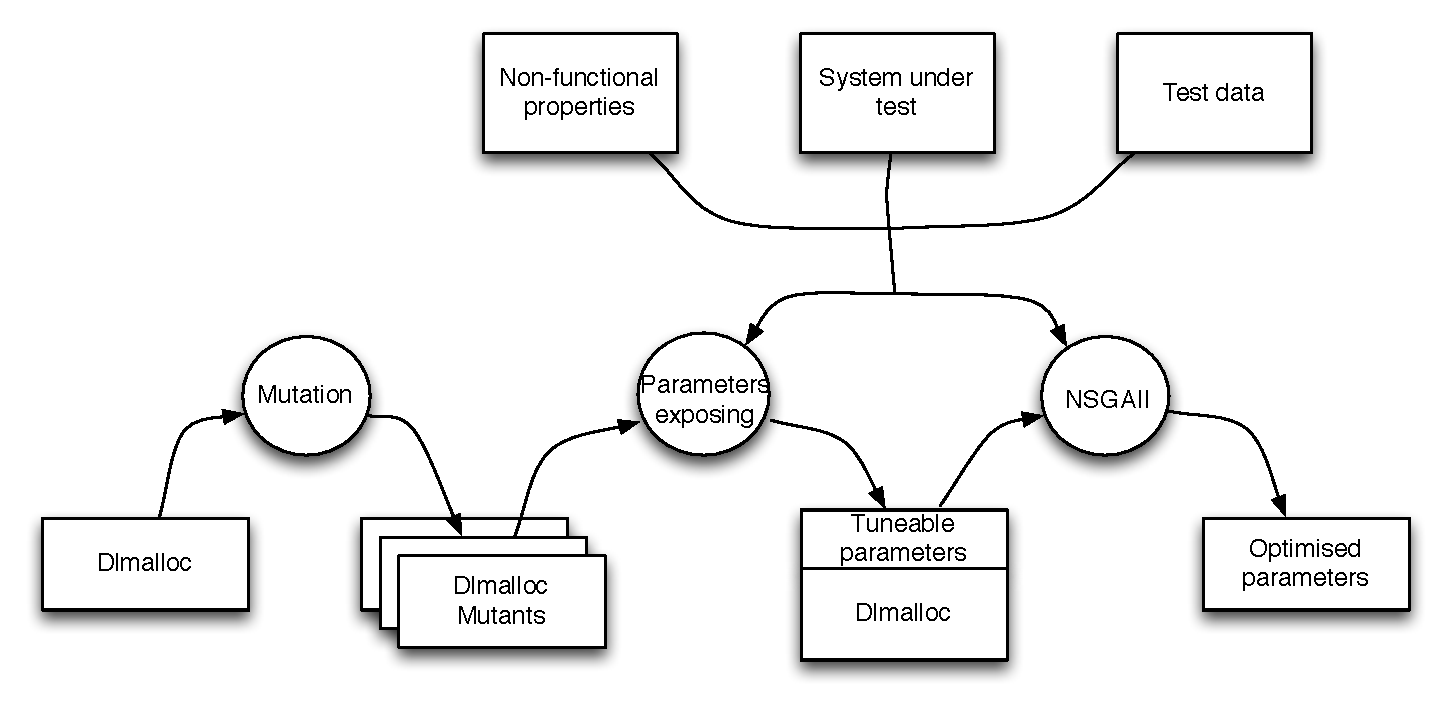
\includegraphics[width=3.2in]{pics/system}
\caption{Deep parameter optimisation workflow}\label{system}
\end{figure}

\subsection{Discoving impact location **}

Besides the Shallow Parameters described in Section \ref{sec_dlmalloc_tunable_parameters}, we want to extend the ability of tuning a program's configuration parameters by exposing more parameters which were hard-coded in the program. In this section, we describe how we define a Deep Parameter and how we choose and expose these Deep Parameters.

We define a Deep Parameter by starting from defining a location from which a Deep Parameter is exposed. A location $L$ is an expression that meets:
\begin{equation}
L: \mbox{CONSTANT} | \mbox{IDENTIFIER} | L\ binary-op\ L | unary-op\ L
\end{equation}
where the $binary-op$ can be a relational operator (>, <, >=, <=, ==, !=), a logical operator (\&\&, ||, !) or an arithmetic operator (+, -, *, /, \%). So a location can be a constant, a variable or an expression derived from other location(s) with an operator. When a location is composed of other location(s) and an operator $op$ and the $op$ is a relational operator or a logical operator, we call it a logical location, otherwise it is an arithmetic location. Then a Deep Parameter is exposed by following the rule:
\begin{equation}
 P(L) = \left\{
  \begin{array}{l l}
    (L) \ xor \ v & \quad \text{if $L$ is a logical location}\\
    (L + v) & \quad \text{if $L$ is an arithmetic location}
  \end{array} \right.,
\end{equation}
in which $v$ is an exposed parameter, or Deep Parameter. After we follow the rule and expose corresponding parameter, users can configure this parameter as a means of taking more control of the program.

Apparently, exposing parameters from all possible locations from a program will give users the maximum capacity to control the behaviour of the program. However, since we want to optimize these Deep Parameters as well as Shallow Parameters on a given test suite, it is impractical to expose and optimize all of possible Deep Parameters. So we firstly need to determine which locations to expose. In theory, we can expose parameter from each legible location and optimize the parameter on a given test suite, to understand how much better performance of the program under optimise we can achieve by tuning this parameter. Formally, $E_{LS}(L)$ is the best performance of a program after exposing and optimizing parameter $v$ from location $L$:
\begin{equation}
E_{LS}(L)=\max_{a} E_T(P(L)|_{v=a}),
\end{equation}
where $E_T()$ is a function which evaluate a program's performance on a given test suite $T$. However, it may needs infinitely large number of evaluations due to the infinite possible values of $a$. Instead, we propose a Mutation-based approach to analyse how likely we could achieve better performance by exposing one parameter than another.

\subsection{Mutation analyse **}
(** old)
In order to obtain the sensitivity information, one simple way is to delete each statement at a time to see how important this statement is to the performance of \emph{dlmalloc}. However, when the statement deleted is consist of a very complicated expression, which variable or operator is more important than others remains unknown. 

A more advanced way to obtain the sensitivity information is via Mutation Operators. Mutation Operators are used in Mutation Testing, which automatically inserts some faults to a target program via Mutation Operators to generate mutants of this program and try to detect those faults using a test suite to see whether the test suite is good enough to reveal program faults. 

In this work, we just use these Mutation Operators to slightly alter \emph{dlmalloc}, in order to understand which piece of source code influences the memory consumption most. We apply both the statement deletion way and Mutation Operator way in the sensitivity analysis and compare their effectiveness, which is reported later. In either way, there are many variants of original \emph{dlmalloc} generated, all of them only differ from the original in at most one statement. We then evaluate and record the performance of these variants on the subject applications and corresponding test suites. This helps us understand the most influential pieces of code in the original \emph{dlmalloc}.

(** fannew)
Mutation Operators are originally used in Mutation Testing to automatically insert artificial faults to a program under test, generating different versions, or mutants, of the original program. These mutants are later test under a given test suite trying to discover those artificial faults as a means of revealing how good the test suite is for detecting real faults. Here we only use Mutation Operators to generate mutants that slightly differ from the original program. According to the Mutation Operators we used, the mutated location $L_m$ can be a constant, a relational operator, a logical operator, an arithmetic operator or a predicate. Then we say a location $L$ involves a mutated location $L_m$ if $L_m$ is a substring of $L$. By this definition, we can approximate $E_{LS}(L)$ by evaluating the best performance of the mutants whose mutated location $L_m$ is involved by $L$. 

Notice that from the same statement, there could be multiple locations by our definition. For example, from the statement $a=b+c$, there are three locations: $L_1:b$, $L_2:c$, $L_3:b+c$. Apparently, exposing parameters from each of them will result in semantically the same program. So if we find exposing parameter from location $L_3$, there is no need to expose more parameters from the other two locations. We say a location $L_a$ covers location $L_b$ if $L_b$ is a substring of $L_a$. For example, locations $L_3$ covers both location $L_1$ and $L_2$ in the previous example. 

(**describe the greedy algorithm we used to choose $k$ location to expose)

(**describe how we apply our approach on the dlmalloc case study, including separately finding best locations to expose with respect to each subject application)

\subsection{Rules to expose deep parameters}

According to the sensitivity information abtained above, we pick the most influential statements and expose part of them as configurable parameters that can be modified at compilation, just like the other existing parameters introduced in section \ref{sec_dlmalloc_tunable_parameters}. These exposed parameters include constants, expressions and predicates. 



\subsection{MultiObjective Paramter optimisation}
\label{sec_nsgaii}
In this work, we apply NSGA II\cite{996017}, a multi-objective Genetic Algorithm, on the searching of the optimal values for those \emph{dlmalloc} parameters list above.
% data representation
Since these parameters can be easily interpreted as integers, we use linear representation to store each candidate, in which each gene is an integer number representing one of the parameters. For mutation, we use different operators according to each gene's legitimate range, while two-point crossover is applied.
% fittness evaluation

Since we need to re-compile \emph{dlmalloc} every time we change the parameters, in order to minimize compilation cost, we only compile \emph{dlmalloc} to a shared object and each application is compiled and linked to that shared object at the beginning of each experiment. In each generation, after new candidates are generated through mutation and crossover operators, each candidate is re-compiled and run with a given subject application. When the performance of the application with each candidate version of \emph{dlmalloc} is collected, an NSGA II style selection is applied to obtain the next generation.
% how to measure time
% how to measure memory

Currently we focus on two non-functional properties: time and memory consumption. \emph{Glibc}'s \emph{wait4} function is used to calculate the cpu time consumed by the application (sum of user time and system time), while we compute the high-water mark of the memory consumption by instrumentation of \emph{dlmalloc}. In this way the memory measured is virtual memory, because the physical pages allocated to an application is not always deterministic but depends on the work load and the system so that measuring the physical memory usage could be hard and misleading.

